\documentclass[a4paper, 12pt]{report}

% Packages
\usepackage[protrusion=false]{microtype}
\usepackage{setspace}

% Language Package
\usepackage[hidelinks]{hyperref}
\usepackage[italian]{babel}
\usepackage[italian]{cleveref}
\usepackage[toc,page]{appendix}
\usepackage{graphicx}
\usepackage[font=footnotesize,labelfont=bf]{caption}

% Environments
\newenvironment{packed_enum}{
\begin{enumerate}
        \setlength{\itemsep}{1pt}
        \setlength{\parskip}{0pt}
        \setlength{\parsep}{0pt}
}{\end{enumerate}}

\newenvironment{packed_itemize}{
\begin{itemize}
        \setlength{\itemsep}{1pt}
        \setlength{\parskip}{0pt}
        \setlength{\parsep}{0pt}
}{\end{itemize}}

% Initialization
\title{HPC Project Report 2023}
\author{Michele Montesi \\
        Matricola: 0000974934 \\
        E-Mail: michele.montesi3@studio.unibo.it}

\date{\today}

\begin{document}
\maketitle

\chapter*{Introduction}
\begin{sloppypar}
This research presents the development of two parallelized versions of the \texttt{sph.c} software, 
implemented using the \textit{OpenMP} and \textit{MPI} libraries, respectively. The objective of the research 
is to evaluate the advantages of using multiprocessor programming.
\end{sloppypar}

\bigskip

\begin{sloppypar}
\noindent
To evaluate the software's performance, a Python script has been created that runs the program with an increasing number of threads for \textit{OpenMP} and processes for \textit{MPI}, starting from 1 and reaching 12, and with a varying number of particles from 1400 to 5700. The script records relevant data in an Excel spreadsheet, from which the average will be calculated. This information will then be used to evaluate the performance.

\bigskip
\noindent
The software has been tested on the \texttt{ISI-Raptor} server.

\end{sloppypar}

{\let\clearpage\relax\chapter*{OpenMP Version}}
\section*{Implementation}
\begin{sloppypar}
  \noindent
  In this implementation of the software, done with \textit{OpenMP}, sections of code that require significant computation have been parallelized using the \texttt{\#pragma omp parallel for} directive.

  \smallskip
  \noindent
  Where necessary, reductions have been made to optimize the performance of the parallelized software.
\end{sloppypar}

\section*{Performance}
\begin{sloppypar}
  \noindent
  From Figure \ref{fig:omp_speedup}, it can be observed that as the number of threads increases, the speedup significantly improves, as indicated by the increasing curve. However, after reaching 8 threads, a saturation phase can be observed, where adding more threads no longer leads to a significant performance improvement. At this point, the use of additional threads may even degrade performance.

  \begin{figure}[ht]
    \centering
    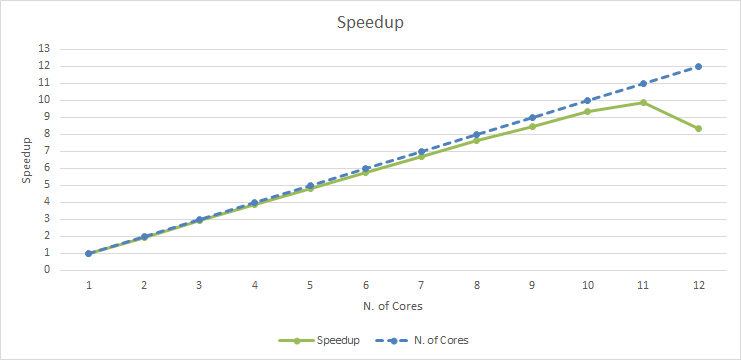
\includegraphics[width=9cm]{img/omp-speedup.png}
    \caption{Speedup of the OpenMP implementation}
    \label{fig:omp_speedup}
  \end{figure}

  \noindent
  From the graph in Figure \ref{fig:omp_sse}, it can be noted that the Strong Scaling Efficiency reaches its maximum peak at around 6 threads, corresponding to an efficiency of about 90% compared to ideal efficiency. After the peak, it starts to decrease, indicating that adding additional threads does not lead to a significant performance improvement and may even cause a degradation of overall performance.

  \begin{figure}[ht]
    \centering
    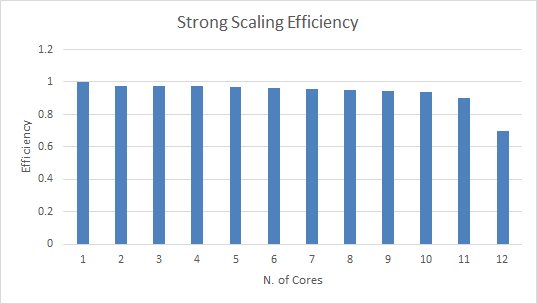
\includegraphics[width=9cm]{img/omp-sse.png}
    \caption{Strong scaling efficiency of the OpenMP implementation}
    \label{fig:omp_sse}
  \end{figure}

  \newpage
  \noindent
  In Figure \ref{fig:omp_wse}, it can be observed that the Weak Scaling Efficiency remains constant as the problem size increases. This indicates that the software efficiently handles problems of varying sizes by distributing the workload among the available CPUs without a significant decrease in performance. This constancy is an indicator of good software scalability. At 12 threads, weak efficiency decreases, indicating that the addition of further threads does not lead to better performance.

  \begin{figure}[ht]
    \centering
    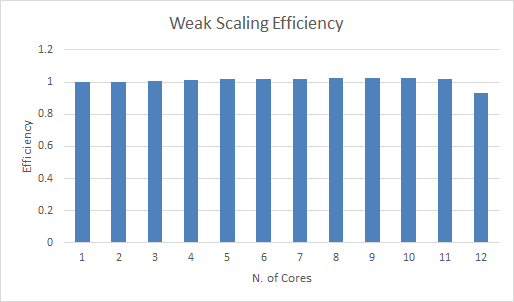
\includegraphics[width=9cm]{img/omp-wse.png}
    \caption{Weak scaling efficiency of the OpenMP implementation}
    \label{fig:omp_wse}
  \end{figure}
\end{sloppypar}

{\let\clearpage\relax\chapter*{MPI Version}}
\section*{Implementation}
For the implementation of the software with MPI, a contiguous MPI\_Datatype has been created to encapsulate the data structure during message exchange. To distribute particles among all processors, an MPI\_Scatterv is performed from process 0. After compute\_density\_pressure and integrate, an MPI\_Allgatherv is called to collect the processed data and redistribute it to all processors again, while compute\_forces is not included as it only acts locally. Finally, after calculating the average velocity of the local particles, an MPI\_Reduce with a summation operator is executed. This result is divided by all processors, obtaining the overall average velocity.

\section*{Performance}
\begin{sloppypar}
  \noindent
  From Figure \ref{fig:mpi_speedup}, it can be observed that the software's performance increases almost linearly as the number of processing units used increases. However, the performance gain in terms of speedup decreases as new processing units are added due to factors such as increased communication time between them, the need for synchronization between processes, and the presence of parts of the software that cannot be parallelized. Moreover, it can be noticed that speedup starts to saturate around 8 cores.

  \begin{figure}[ht]
    \centering
    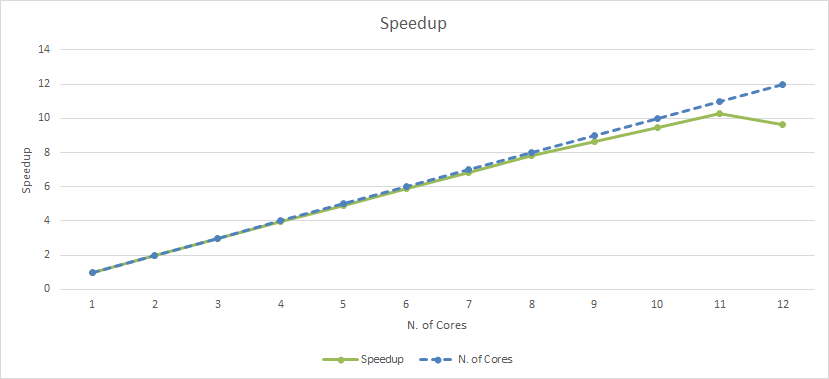
\includegraphics[width=9cm]{img/mpi-speedup.png}
    \caption{Speedup of the MPI implementation}
    \label{fig:mpi_speedup}
  \end{figure}

  \noindent
  From the graph in Figure \ref{fig:mpi_sse}, it is evident that the Strong Scaling Efficiency reaches its peak at around 6 cores, achieving an efficiency of approximately 90% compared to ideal efficiency. However, after the peak, efficiency starts to decrease, indicating that adding more cores does not lead to a significant performance improvement and may even worsen performance in some cases.

  \begin{figure}[ht]
    \centering
    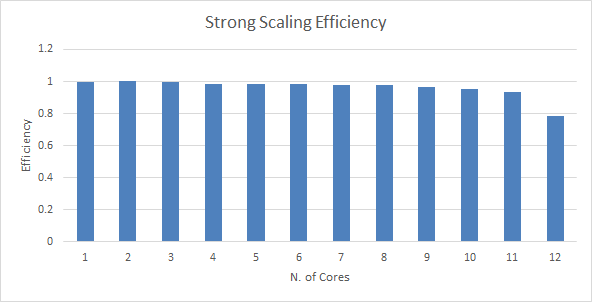
\includegraphics[width=9cm]{img/mpi-sse.png}
    \caption{Strong scaling efficiency of the MPI implementation}
    \label{fig:mpi_sse}
  \end{figure}

  \newpage
  \noindent
  The graph of Weak Scaling Efficiency (Figure \ref{fig:mpi_wse}) shows that the efficiency of the software remains constant as the problem size varies. This suggests that the software efficiently handles problems of varying sizes by distributing the workload among the available CPUs without a significant decrease in performance. This is an indicator of good software scalability. However, the addition of additional cores beyond 12 results in decreased weak efficiency, indicating that the use of additional resources does not translate into better performance.

  \begin{figure}[ht]
    \centering
    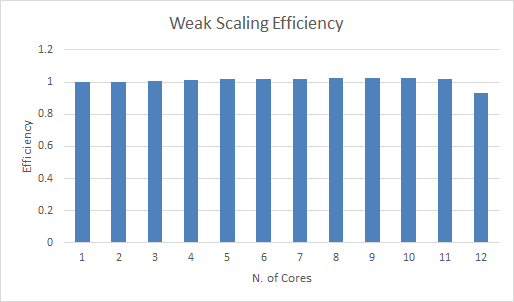
\includegraphics[width=9cm]{img/mpi-wse.png}
    \caption{Weak scaling efficiency of the MPI implementation}
    \label{fig:mpi_wse}
  \end{figure}

\end{sloppypar}

\chapter*{Conclusions}
\begin{sloppypar}
  \noindent
  The implementation of the software with OpenMP has led to significant performance improvements, as indicated by the speedup graph as a function of the number of threads. It was observed that increasing the number of threads significantly improved performance up to a certain point, after which the positive effect saturated, indicating that using additional threads could even degrade performance. Strong scaling efficiency was rather high for cases with a low number of threads but decreased as the number of threads increased. Weak scaling efficiency was good and consistent as the number of processors varied.

  \bigskip
  \noindent
  The implementation with MPI resulted in a significant reduction in execution times compared to the sequential version of the software, as indicated by the speedup graph as a function of the number of processors. It was observed that strong scaling efficiency was very high for all cases analyzed, indicating good scalability of the software. Weak scaling efficiency was good and consistent as the number of processors varied.

  \bigskip
  \noindent
  In conclusion, the implementation of the software with OpenMP and MPI led to significant performance improvements compared to the sequential version. The OpenMP approach is particularly effective for problems of limited size and with a small number of threads, while the MPI approach is more efficient for larger problems and with a high number of processors.
\end{sloppypar}
  
\end{document}
